\documentclass{standalone}
\usepackage{tikz}
\usetikzlibrary{arrows.meta,babel,positioning}
\tikzset{%
    >={Latex[width=2mm,length=2mm]},
    base/.style = {
        rectangle, rounded corners, draw=black, minimum width=4cm,
        minimum height=1cm, text centered, font=\sffamily
    },
    startLoop/.style = {base, fill=blue!30},
    transition/.style = {circle, draw, fill=green!30},
    process/.style = {base, minimum width=2.5cm, fill=orange!15, font=\ttfamily},
}
\begin{document}
    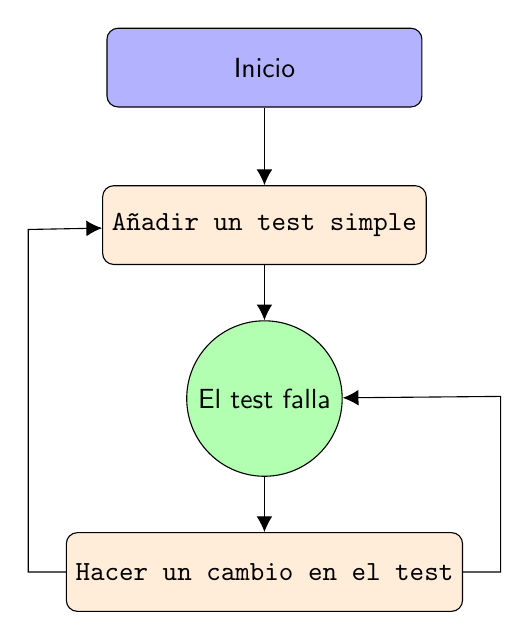
\begin{tikzpicture}[
        node distance=1.5cm,
        every node/.style={fill=white, font=\sffamily},
        align=center
    ]
        % Nodes position
        \node (start)         [startLoop]
                                {Inicio};
        \node (addTest)       [process, below of=start, yshift=-0.5cm]
                                {Añadir un test simple};
                                
        \node (testFail)     [transition, below of=addTest, yshift=-20]
                                {El test falla};
                                
        \node (makeChange)    [process, below of=testFail, yshift=-20]
                                {Hacer un cambio en el test};
                            
        % Arrow specification
        \draw[->]         (start) -- (addTest);
        \draw[->]       (addTest) -- (testFail);
        \draw[->] (testFail) -- (makeChange);
        \draw[->]  (makeChange) -- ++(3, 0) -- ++(0, 2.23) -- (testFail);
        \draw[->]        (makeChange) -- ++(-3,0) -- ++(0, 4.35) -- (addTest);
    \end{tikzpicture}
\end{document}